
%(BEGIN_QUESTION)
% Copyright 2006, Tony R. Kuphaldt, released under the Creative Commons Attribution License (v 1.0)
% This means you may do almost anything with this work of mine, so long as you give me proper credit

En blandetank i et avløpsrenseanlegg mottar vann med varierende pH-nivå, og reguleringssystemets oppgave er å holde pH i utløpet rundt 7 (nøytral) ved å tilsette syre eller lut etter behov. Hvis innkommende vann er for surt (pH under 7), skal systemet tilføre mer lut. Hvis innkommende vann er for basisk (pH over 7), skal systemet tilføre mer syre:

$$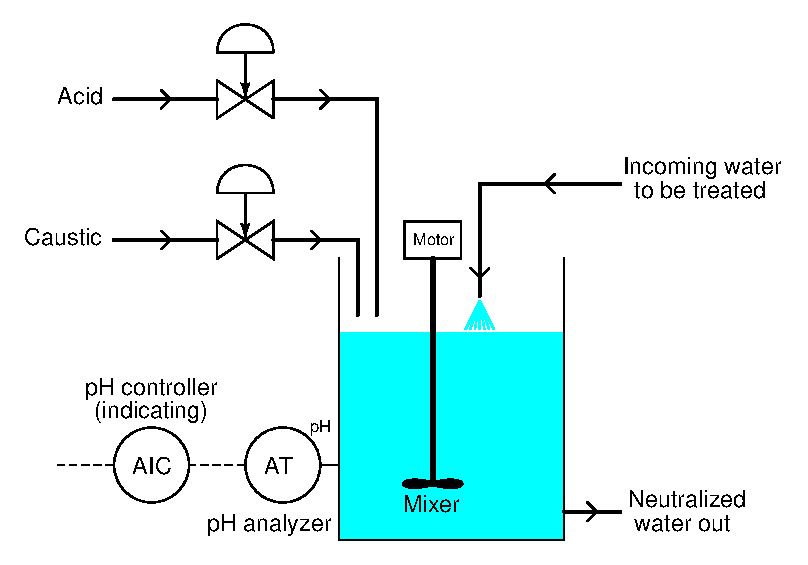
\includegraphics[width=15.5cm]{i01395x01.eps}$$

Hvis innkommende pH er under 7 (sur), må reguleringssystemet åpne lutventilen for å øke pH i utløpet. Hvis innkommende pH er over 7 (basisk), må systemet åpne syreventilen for å senke pH i utløpet. Det ville imidlertid være sløsing å tilføre både syre {\it og} lut til blandetanken samtidig, siden de vil motvirke hverandre.

Hvordan er det mulig å styre syre-/lutventilene på denne måten fra én enkelt regulator? Tegn inn en løsning i P\&ID-diagrammet over for å vise hvordan du ville gjort det.

\vskip 20pt \vbox{\hrule \hbox{\strut \vrule{} {\bf Forslag til sokratisk diskusjon} \vrule} \hrule}

\begin{itemize}
\item{} En god problemløsningsmetode i tilfeller der vi må bestemme retningen på en endring, er å vurdere {\it grenseverdier}. I stedet for å spørre hva som skjer hvis pH endrer seg litt, spør vi hva som skjer hvis pH endrer seg {\it dramatisk}. Forklar hvordan denne metoden kan brukes på dette systemet, der vi må bestemme nødvendig regulatorvirkning og sekvensering av sluttelementene.
\item{} Hva representerer pilsymbolene på ventilspindlene?
\item{} Identifiser konsekvensen av tap av instrumentluft til reguleringsventilene -- hva vil skje med pH i utløpet?
\item{} Identifiser konsekvensen av en avbrutt (feilåpen) 4-20 mA-kabel i løsningen du foreslår -- hva vil skje med pH i utløpet?
\item{} Identifiser alternative split-range-sekvenseringskonfigurasjoner (andre enn den du foreslo i svaret ditt).
\end{itemize}

\underbar{file i01395}
%(END_QUESTION)





%(BEGIN_ANSWER)

Dette er én måte å koble ventilene sammen på som et split-range-par:

$$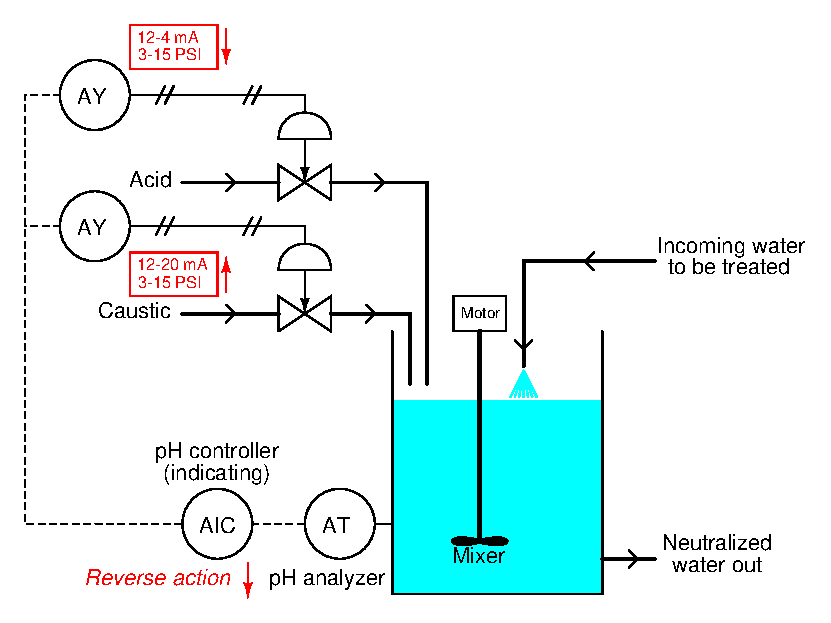
\includegraphics[width=15.5cm]{i01395x02.eps}$$

%(END_ANSWER)





%(BEGIN_NOTES)

Dette er formen for split-ranging vi trenger, gitt en {\it reversvirkende} regulator:

$$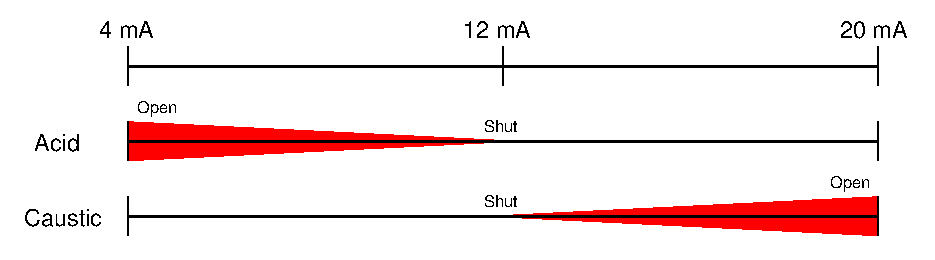
\includegraphics[width=15.5cm]{i01395x03.eps}$$

De to I/P-transduserne (``AY''-enheter) vil begge ha utgangsområde 3-15 PSI, men den ene får inngangsområde 4-12 mA mens den andre får inngangsområde 12-20 mA.

\vskip 10pt

En annen mulighet er å bruke én enkelt I/P-transduser og forsterke utgangen med to pneumatiske multiplikatorreleer: ett med inngangsområde 3-9 PSI og utgangsområde 3-15 PSI, og ett med inngangsområde 9-15 PSI og utgangsområde 3-15 PSI. Teknikken med to pneumatiske forsterkningsreleer gir imidlertid mest mening når regulatorutgangen er pneumatisk. Hvis regulatoren er elektronisk, er det mer hensiktsmessig å bruke to I/P-transdusere i stedet for én I/P-transduser og to forsterkningsreleer.

For øvrig er den generiske bokstaven for målt variabel i et analytisk (kjemimålende) instrument ``A'', og siden pH er en kjemisk måling, er ``AT'' en passende betegnelse for en pH-transmitter. Legg merke til bokstavene ``pH'' øverst til høyre ved transmittersymbolet, plassert der for å presisere transmitterens funksjon ytterligere. Det er imidlertid også riktig å bruke bokstavene ``pH'' direkte for å merke instrumenter i en pH-sløyfe. Vi kunne derfor ha merket analysatoren (transmitteren) som ``pHT'' og den indikerende regulatoren som ``pHIC'' i stedet for ``AT'' og ``AIC.'' På samme måte kunne de to I/P-transduserne ha vært merket ``pHY'' i stedet for ``AY.''

%INDEX% Final Control Elements, valve: split ranging
%INDEX% Process: water pH neutralization (generic)

%(END_NOTES)

